\section{The Cut-Matching Game}
Definition:
\begin{enumerate}
    \item \textbf{Sparsity of a vertex subset}: Given $\emptyset \subset S \subset V$, the conductance $\psi(S) := \frac{|E(S, V \backslash S)|}{\min \{|S|, |V\setminus S|\}}$. This is different to the conductance $\phi(S)$ in the denominator. Since $\vol{S} \ge |S|$, it is guaranteed that $\psi(S) \ge \phi(S)$.
    \item \textbf{Sparsity of a graph}: $\psi(G):= \min_{\emptyset \subset S \subset V} \psi(S)$. We say $G$ is a $\psi$-expander w.r.t. sparsity iff $\psi(G) \ge \psi$. The cut that achieves the minimum is called the sparsest cut.
\end{enumerate}

The cut-matching game is an algorithm that involves interaction of the cut player and the matching player, designed to follow a specific strategy, so that the result of such a game could certfify the sparsity of a graph.

\subsection{Certifying via Embedding}

Given graphs $H$ and $G$ defined on the same vertex set, we say a function is an embedding of $H$ into $G$ if it maps each edge $(u,v) \in H$ to a $u$-to-$v$ path in $G$. We define the congestion of such an embedding to be the maximum number of times that any edge in $G$ appears on any embedding path.

\textbf{Property}: given a $\psi$-expander graph $H$ and an embedding of $H$ into $G$ with congestion $C$, then $G$ is a $\psi/C$-expander.
\begin{proof}
    For any cut $(S, V\setminus S)$ such that $|S|\le n/2$, we have $|E_H(S, V\setminus S)| \ge \psi |S|$. For every edge $(u,v)$ in $|E_H(S, V\setminus S)|$, there is a path from $u$ to $v$ in $G$ which crosses the cut. Since each edge crossing the cut can be used at most $C$ times, we have that $|E_G(S, V\setminus S)| \ge \psi |S|/C$, which implies that $G$ is a $\psi/C$-expander.
\end{proof}

\subsection{Certifying $\psi$-expanders via Max Flows}

Theorem 14.1.1. There is an algorithm CertifyOrCut$(G, \psi)$ that given a graph $G$ and a parameter $0<\psi \leq 1$, either:
\begin{itemize}
    \item Certifies that $G$ is a $\Omega\left(\psi / \log ^{2} n\right)$-expander w.r.t. sparsity.
    \item Presents a cut $S$ such that $\psi(S) \leq O(\psi)$.
\end{itemize}
The algorithm runs in time $O\left(\log^{2} n\right) \cdot T_{\text {max\_flow }}(G)+\tilde{O}(m)$ where $T_{\text{max-flow }}(G)$ is the time it takes to solve a Max Flow problem on $G$.

Illustration of one iteration of the Algorithm:

\begin{center}
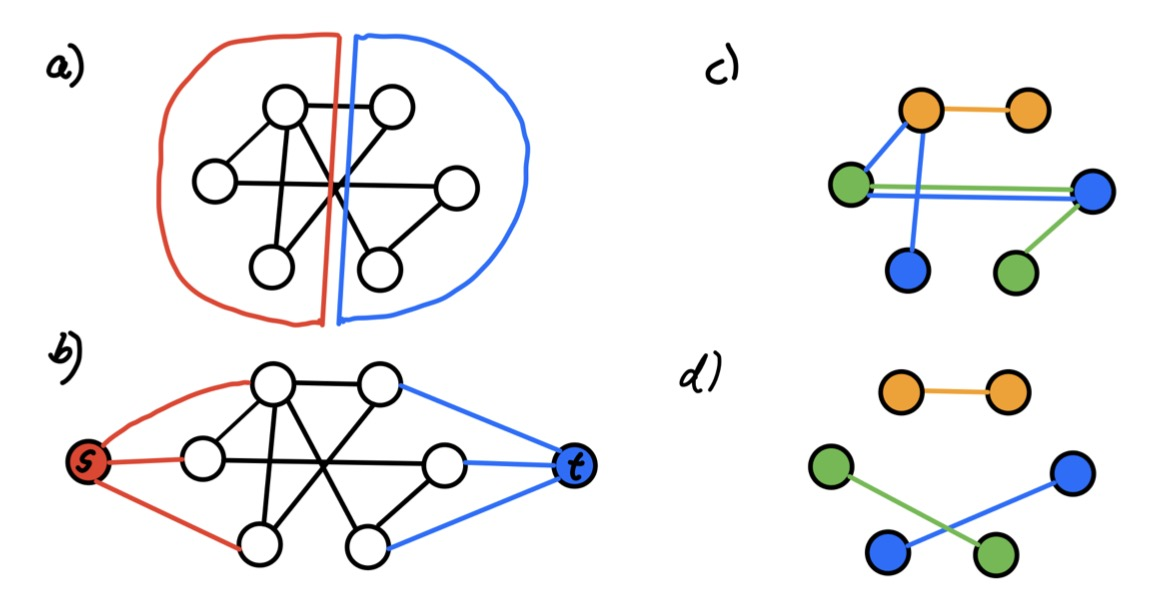
\includegraphics[width=.6\columnwidth]{imgs/cut-match.png}
\end{center}

 In a), a bi-partition $(S_i, \bar{S_i})$ of $V$ is found (requires random walk on $G$). In b), the bi-partition is used to obtain a flow problem where we inject one unit of flow to each vertex in $S_i$ via super-source $s$ and extract one unit of flow from each vertex in $\bar{S_i}$ via super-sink $t$. Every edge is set to have capacity $1/\psi$. Then we solve this problem to get a flow $f$ with $\val(f)=n/2$. If such flow does not exist, then we return the min-cut of this flow problem, removing the dummy source and sink.  c) If such flow exists, we construct a path flow decomposition. For each path, the first vertex is in $S$ and the last vertex in $\bar{S}$. d) We find $M_{i}$ to be the one-to-one matching between endpoints in $S$ and $\bar{S}$ defined by the path flows.

 It can be proven that after $T=\Theta(\log^2 n)$ iterations, the union of the $T$ matchings is a $1/2$-expander and $G$ can be embedded into $H$ with congestion $O(\log^2 n / \psi)$, which certifies that $G$ is a $O(\psi / \log^2 n)$-expander. If one of the iterations presents a cut, then it can be proven that the sparsity of this cut is $O(\psi)$.